\section{Quantitative Comparison}
Here goes the quantitative comparison.

\subsection{Bandwidth}
Measure number of bytes transferred between device and proxy.
More packet to send = more energy consumption

\textbf{First experiment:} Single transaction (non-coap,con-coap,coap over tcp).
\\ \\
	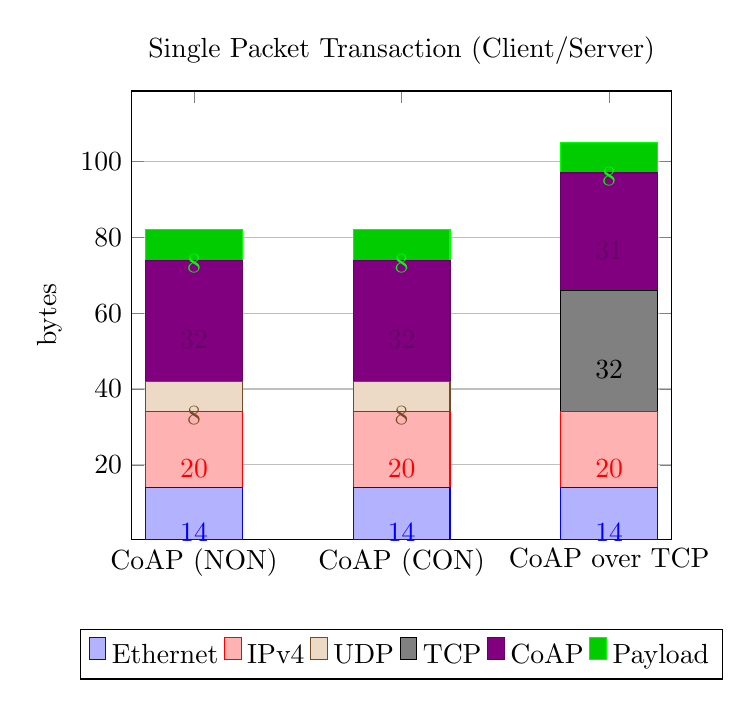
\begin{tikzpicture}
	\begin{axis}[
	 title={Single Packet Transaction (Client/Server)},
	ybar stacked,
	%ymax=50,
	ymajorgrids,
	bar width=35pt,
	%width=250pt,
	nodes near coords, 
	 %nodes near coords={\pgfmathprintnumber\pgfplotspointmeta \%},
	nodes near coords align={anchor=north},%Move values in bar
	every node near coord/.style={
	},
	enlargelimits=0.15,
	legend style={at={(0.5,-0.20)},
		anchor=north,legend columns=-1},
	%width=0.8*\textwidth,
	ylabel={bytes},
	symbolic x coords={CoAP (NON), CoAP (CON), CoAP over TCP},
	xtick=data,
	%legend pos= north east,
	%x tick label style={rotate=45,anchor=east},
	]
	%ethernet
	\addplot+[ybar] plot coordinates {(CoAP (NON),14) (CoAP (CON),14) 
		(CoAP over TCP,14) };
	%ipv4
	\addplot+[ybar] plot coordinates {(CoAP (NON),20) (CoAP (CON),20) 
		(CoAP over TCP,20) };
	%udp
	\addplot+[ybar] plot coordinates {(CoAP (NON),8) (CoAP (CON),8) 
		(CoAP over TCP,0) };
	%tcp
	\addplot+[ybar] plot coordinates {(CoAP (NON),0) (CoAP (CON),0) 
		(CoAP over TCP,32) };
	%coap 
	\addplot+[ybar] plot coordinates {(CoAP (NON),32) (CoAP (CON),32) 
		(CoAP over TCP,31) };
	%payload
	\addplot+[ybar] plot coordinates {(CoAP (NON),8) (CoAP (CON),8) 
		(CoAP over TCP,8) };
	
	\legend{\strut Ethernet, \strut IPv4, \strut UDP, \strut TCP , \strut CoAP, \strut Payload}
	\end{axis}
	\end{tikzpicture}

CoAP over TCP is 1 byte shorter than CoAP over UDP because of the MessageID-field (2 byte) is removed and replaced with the Length-field (1 byte). 

\textbf{Second experiment:} Complete scenario (non-coap,con-coap,coap over tcp)
Transmitting packets for 30 minutes with a 30 seconds interval, and thereby we have a complete scenario where we can get information about how bandwith transmitting and receiving data requires.

Results are in Wireshark files with the three categories (CoAP (NON), CoAP (CON), CoAP over TCP)

\textbf{En god ide er at maale energiforbruge / beregne det i joule. Giver et konkret svar om den kan bruges i specifikke typer af constraint devices}

\subsection{Packet-loss}
Use the NetEM tool for emulating package-loss.
More lost packet = more packet to send = more energy consumption

\subsection{Latency}
Measure RTT values %which is the time from establishing the connection to receiving the acknowledgement.
More latency = less time to sleep = more energy consumption

Undersøg hvad den timestamp i TCP bruges til.

\textbf{First experiment:} Single transaction (non-coap,con-coap,coap over tcp).
\\ \\
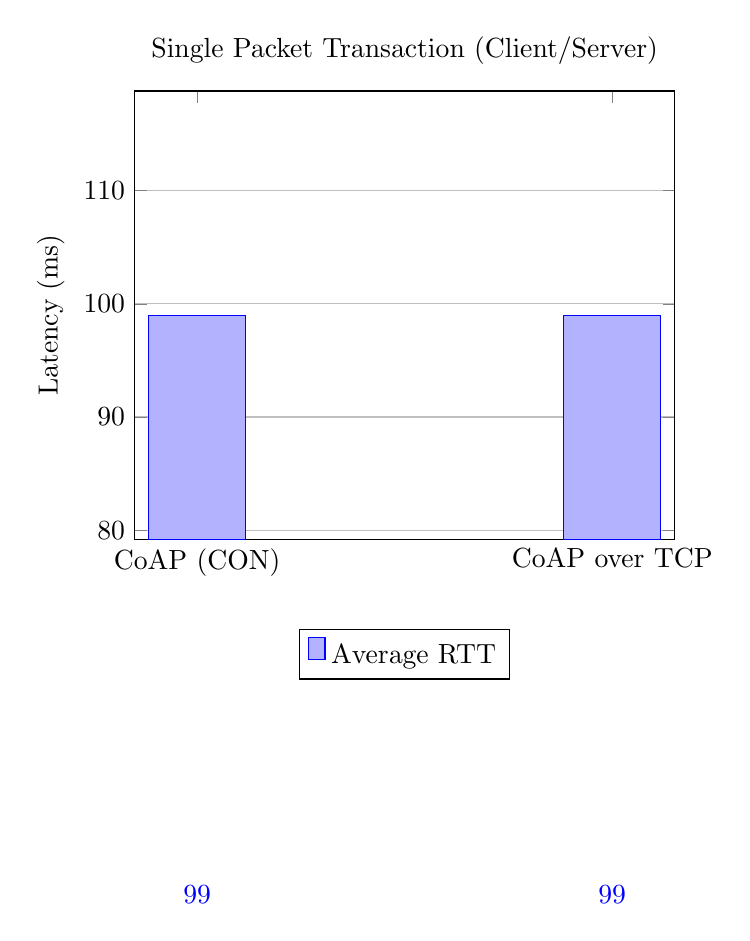
\begin{tikzpicture}
\begin{axis}[
title={Single Packet Transaction (Client/Server)},
ybar stacked,
%ymax=50,
ymajorgrids,
bar width=35pt,
%width=250pt,
nodes near coords, 
%nodes near coords={\pgfmathprintnumber\pgfplotspointmeta \%},
nodes near coords align={anchor=north},%Move values in bar
every node near coord/.style={
},
enlargelimits=0.15,
legend style={at={(0.5,-0.20)},
	anchor=north,legend columns=-1},
%width=0.8*\textwidth,
ylabel={Latency (ms)},
symbolic x coords={CoAP (CON), CoAP over TCP},
xtick=data,
%legend pos= north east,
%x tick label style={rotate=45,anchor=east},
]
%ethernet
\addplot+[ybar] plot coordinates { (CoAP (CON),99) 
	(CoAP over TCP,99) };


\legend{\strut Average RTT}
\end{axis}
\end{tikzpicture}
Spredning/fordeling/varians af delay variations 

\subsection{Memory consumption}
Flyt den del til et afsnit med prototype implementation (før resultaterne)
How much memory usage...


